% Options for packages loaded elsewhere
\PassOptionsToPackage{unicode}{hyperref}
\PassOptionsToPackage{hyphens}{url}
%
\documentclass[
  12pt,
]{article}
\usepackage{amsmath,amssymb}
\usepackage{iftex}
\ifPDFTeX
  \usepackage[T1]{fontenc}
  \usepackage[utf8]{inputenc}
  \usepackage{textcomp} % provide euro and other symbols
\else % if luatex or xetex
  \usepackage{unicode-math} % this also loads fontspec
  \defaultfontfeatures{Scale=MatchLowercase}
  \defaultfontfeatures[\rmfamily]{Ligatures=TeX,Scale=1}
\fi
\usepackage{lmodern}
\ifPDFTeX\else
  % xetex/luatex font selection
    \setmainfont[]{Times New Roman}
\fi
% Use upquote if available, for straight quotes in verbatim environments
\IfFileExists{upquote.sty}{\usepackage{upquote}}{}
\IfFileExists{microtype.sty}{% use microtype if available
  \usepackage[]{microtype}
  \UseMicrotypeSet[protrusion]{basicmath} % disable protrusion for tt fonts
}{}
\makeatletter
\@ifundefined{KOMAClassName}{% if non-KOMA class
  \IfFileExists{parskip.sty}{%
    \usepackage{parskip}
  }{% else
    \setlength{\parindent}{0pt}
    \setlength{\parskip}{6pt plus 2pt minus 1pt}}
}{% if KOMA class
  \KOMAoptions{parskip=half}}
\makeatother
\usepackage{xcolor}
\usepackage[margin=1in]{geometry}
\usepackage{longtable,booktabs,array}
\usepackage{calc} % for calculating minipage widths
% Correct order of tables after \paragraph or \subparagraph
\usepackage{etoolbox}
\makeatletter
\patchcmd\longtable{\par}{\if@noskipsec\mbox{}\fi\par}{}{}
\makeatother
% Allow footnotes in longtable head/foot
\IfFileExists{footnotehyper.sty}{\usepackage{footnotehyper}}{\usepackage{footnote}}
\makesavenoteenv{longtable}
\usepackage{graphicx}
\makeatletter
\def\maxwidth{\ifdim\Gin@nat@width>\linewidth\linewidth\else\Gin@nat@width\fi}
\def\maxheight{\ifdim\Gin@nat@height>\textheight\textheight\else\Gin@nat@height\fi}
\makeatother
% Scale images if necessary, so that they will not overflow the page
% margins by default, and it is still possible to overwrite the defaults
% using explicit options in \includegraphics[width, height, ...]{}
\setkeys{Gin}{width=\maxwidth,height=\maxheight,keepaspectratio}
% Set default figure placement to htbp
\makeatletter
\def\fps@figure{htbp}
\makeatother
\setlength{\emergencystretch}{3em} % prevent overfull lines
\providecommand{\tightlist}{%
  \setlength{\itemsep}{0pt}\setlength{\parskip}{0pt}}
\setcounter{secnumdepth}{5}
% definitions for citeproc citations
\NewDocumentCommand\citeproctext{}{}
\NewDocumentCommand\citeproc{mm}{%
  \begingroup\def\citeproctext{#2}\cite{#1}\endgroup}
\makeatletter
 % allow citations to break across lines
 \let\@cite@ofmt\@firstofone
 % avoid brackets around text for \cite:
 \def\@biblabel#1{}
 \def\@cite#1#2{{#1\if@tempswa , #2\fi}}
\makeatother
\newlength{\cslhangindent}
\setlength{\cslhangindent}{1.5em}
\newlength{\csllabelwidth}
\setlength{\csllabelwidth}{3em}
\newenvironment{CSLReferences}[2] % #1 hanging-indent, #2 entry-spacing
 {\begin{list}{}{%
  \setlength{\itemindent}{0pt}
  \setlength{\leftmargin}{0pt}
  \setlength{\parsep}{0pt}
  % turn on hanging indent if param 1 is 1
  \ifodd #1
   \setlength{\leftmargin}{\cslhangindent}
   \setlength{\itemindent}{-1\cslhangindent}
  \fi
  % set entry spacing
  \setlength{\itemsep}{#2\baselineskip}}}
 {\end{list}}
\usepackage{calc}
\newcommand{\CSLBlock}[1]{\hfill\break\parbox[t]{\linewidth}{\strut\ignorespaces#1\strut}}
\newcommand{\CSLLeftMargin}[1]{\parbox[t]{\csllabelwidth}{\strut#1\strut}}
\newcommand{\CSLRightInline}[1]{\parbox[t]{\linewidth - \csllabelwidth}{\strut#1\strut}}
\newcommand{\CSLIndent}[1]{\hspace{\cslhangindent}#1}
\usepackage{tcolorbox}
\usepackage{amssymb}
\usepackage{yfonts}
\usepackage{bm}
\usepackage{titlesec}
\usepackage{kbordermatrix}


\newtcolorbox{greybox}{
  colback=white,
  colframe=blue,
  coltext=black,
  boxsep=5pt,
  arc=4pt}
  
\newcommand{\sectionbreak}{\clearpage}

 
\newcommand{\ds}[4]{\sum_{{#1}=1}^{#3}\sum_{{#2}=1}^{#4}}
\newcommand{\us}[3]{\mathop{\sum\sum}_{1\leq{#2}<{#1}\leq{#3}}}

\newcommand{\ol}[1]{\overline{#1}}
\newcommand{\ul}[1]{\underline{#1}}

\newcommand{\amin}[1]{\mathop{\text{argmin}}_{#1}}
\newcommand{\amax}[1]{\mathop{\text{argmax}}_{#1}}

\newcommand{\ci}{\perp\!\!\!\perp}

\newcommand{\mc}[1]{\mathcal{#1}}
\newcommand{\mb}[1]{\mathbb{#1}}
\newcommand{\mf}[1]{\mathfrak{#1}}

\newcommand{\eps}{\epsilon}
\newcommand{\lbd}{\lambda}
\newcommand{\alp}{\alpha}
\newcommand{\df}{=:}
\newcommand{\am}[1]{\mathop{\text{argmin}}_{#1}}
\newcommand{\ls}[2]{\mathop{\sum\sum}_{#1}^{#2}}
\newcommand{\ijs}{\mathop{\sum\sum}_{1\leq i<j\leq n}}
\newcommand{\jis}{\mathop{\sum\sum}_{1\leq j<i\leq n}}
\newcommand{\sij}{\sum_{i=1}^n\sum_{j=1}^n}
	
\ifLuaTeX
  \usepackage{selnolig}  % disable illegal ligatures
\fi
\usepackage{bookmark}
\IfFileExists{xurl.sty}{\usepackage{xurl}}{} % add URL line breaks if available
\urlstyle{same}
\hypersetup{
  pdfauthor={Jan de Leeuw - University of California Los Angeles},
  hidelinks,
  pdfcreator={LaTeX via pandoc}}

\title{Smacof at 50: A Manual\\
Part 2: Metric Smacof}
\author{Jan de Leeuw - University of California Los Angeles}
\date{Started December 12 2022, Version of May 03, 2024}

\begin{document}
\maketitle
\begin{abstract}
TBD
\end{abstract}

{
\setcounter{tocdepth}{3}
\tableofcontents
}
\textbf{Note:} This is a working manuscript which will be expanded/updated
frequently. All suggestions for improvement are welcome. All Rmd, tex,
html, pdf, R, and C files are in the public domain. Attribution will be
appreciated, but is not required. The files can be found at
\url{https://github.com/deleeuw} in the repositories smacofCode, smacofManual,
and smacofExamples.

\section{Introduction}\label{introduction}

In this part of the manual we discuss metric MDS, and the program
smacofAC.

\section{Bells and Whistles}\label{bells-and-whistles}

There are two options, \emph{bounds} and \emph{constant}, to make smacofAC more interesting and more widely applicable. Using these options the metric MDS problem becomes minimization of
\[
\sigma(X,\hat D)=\sum\sum w_{ij}(\hat d_{ij}-d_{ij}(X))^2
\]
over both \(X\) and \(\hat D\), allowing some limited ``metric'' transformations of the data \(\Delta\).
The four ``metric'' types of transformations are

\begin{enumerate}
\def\labelenumi{\arabic{enumi}.}
\tightlist
\item
  type AC1: if bounds = 1 and constant = 1 \(\delta^-_{ij}+c\leq\hat d_{ij}\leq\delta^+_{ij}+c\) for some \(c\),
\item
  type AC2: if bounds = 0 and constant = 1 \(\hat d_{ij}=\delta_{ij}+c\) for some \(c\),
\item
  type AC3: if bounds = 1 and constant = 0 \(\delta^-_{ij}\leq\hat d_{ij}\leq\delta^+_{ij}\),
\item
  type AC4: if bounds = 0 and constant = 0 \(\hat d_{ij}=\delta_{ij}\).
\end{enumerate}

In addition all four types require that \(\hat d_{ij}\geq 0\) for all \((i,j)\). Note that for
types AC1 and AC2 the data \(\Delta\) do not need to be non-negative. In fact,
the original motivation for the additive constant in classical scaling (Messick and Abelson (1956))
was that Thurstonian analysis of paired or triadic comparisons produced dissimilarities on an interval scale, and thus could very well include negative values. The non-negativity requirement
for \(\hat D\) means in the case of AC2 that \(c\geq-\min\delta_{ij}\). For AC1 it means
\(c\geq-\min\delta_{ij}^+\).

In AC1 and AC3 there is no mention of \(\Delta\), which means
the bounds \(\Delta^-\) and \(\Delta^+\) are actually the data. We could
collect dissimilarity data by asking subjects for interval judgments. Instead
of a rating scale with possible responses from one to ten we could ask
for a mark on a line between zero and ten, and then interpret the
marks as a choice of one of the intervals \([k, k+1]\). These finite precision
or interval type of data could even come from physical measurements of distances.
Thus the bounds parameter provides one way to incorporate uncertainty into MDS, similar to interval analysis, fuzzy computing, or soft computing.

makes sense to choose both \(\Delta^-\) and \(\Delta^+\) to be monotone with \(\Delta\),
although there is no requirement to do so.

\subsection{Type AC2}\label{type-ac2}

Cooper (1972)

\subsection{Type AC1}\label{type-ac1}

Of the four regression problems only the one with bounds = 1 and constant = 1 is non-trivial.
It may help to give an example of what it actually requires. We use the De Gruijter example
with \(\delta_{ij}^-=\delta_{ij}-1\) and \(\delta_{ij}^+=\delta_{ij}-1\).

\begin{verbatim}
##       KVP PvdA  VVD  ARP  CHU  CPN  PSP   BP
## PvdA 5.63                                   
## VVD  5.27 6.72                              
## ARP  4.60 5.64 5.46                         
## CHU  4.80 6.22 4.97 3.20                    
## CPN  7.54 5.12 8.13 7.84 7.80               
## PSP  6.73 4.59 7.55 6.73 7.08 4.08          
## BP   7.18 7.22 6.90 7.28 6.96 6.34 6.88     
## D66  6.17 5.47 4.67 6.13 6.04 7.42 6.36 7.36
\end{verbatim}

The distances are
taken from the Torgerson solution.

The Shepard plot is in figure \ref{fig:bandplot}. The two
lines are connecting the \(\delta_{ij}^-\) and the \(\delta_{ij}^+\), i.e.~they give
the bounds for \(c=0\). In our example the lines are parallel, because \(\delta_{ij}^+-\delta_{ij}^-=2\) for all \((i,j)\), but in general this may not be the case.
We could, for example, set \(\delta_{ij}^+=(1+\alpha)\delta_{ij}\) and
\(\delta_{ij}^-=(1-\alpha)\delta_{ij}\), in which case the region between \(\delta^-\)
and \(\delta^+\) is like a trumpet.
The bounds \(\delta_{ij}^-\) and \(\delta_{ij}^+\) are not necessarily a monotone function of \(\delta\), in fact there may not even be a \(\delta\). Also note that the \(\delta_{ij}^-\) are not necessarily non-negative.

The points between the two lines do not contribute to the loss, and
the points outside the strip contribute by how much they are outside.

\begin{figure}

{\centering 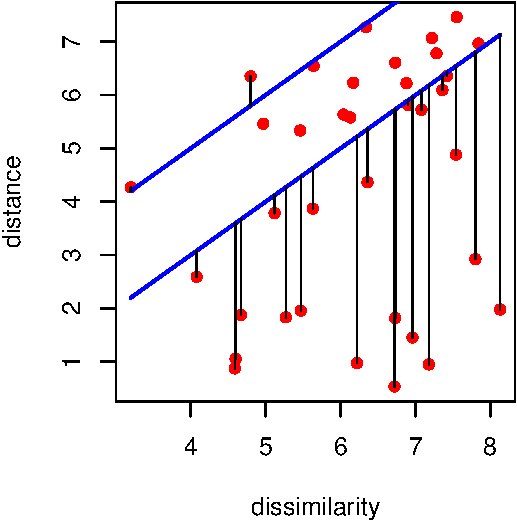
\includegraphics{smacofAC_files/figure-latex/bandplot-1} 

}

\caption{De Gruijter Shepard Plot}\label{fig:bandplot}
\end{figure}

By varying \(c\) we shift the region between the two parallel lines upwards or downwards. The width of the region, or more generally the shape, always remains the same, because it is determined by the difference of \(\delta^+\) and \(\delta^-\) and does not depend on \(c\). The
optimal \(c\) is the shift for which the red \((\delta_{ij},d_{ij}(X))\) points are optimally within the strip between the \(\delta^-\) and \(\delta^+\) lines. This is in the least squares sense, which
means that we minimize the horizontal squared distances from the points outside the strip to the
\(\delta^-\) and \(\delta^+\) lines.

Let's formalize this. Define
\begin{equation}
\phi_{ij}(c):=\min_{\delta_{ij}\geq 0}\{(\delta_{ij}-d_{ij}(X))^2\mid \delta^-_{ij}+c\leq\delta_{ij}\leq\delta^+_{ij}+c\}
\label{eq:phiijdef}
\end{equation}
and
\begin{equation}
\phi(c):=\sum\sum w_{ij}\phi_{ij}(c)
\label{eq:phidef}
\end{equation}
The constraints are consistent if \(\delta_{ij}^++c\geq 0\), i.e.~if \(c\geq c_0:=-\min\delta_{ij}^+\).
The regression problem is to minimize \(\phi\) over \(c\geq c_0:=-\min\delta_{ij}^+\). At first sight it seems this we should require the stricter bound \(c\geq-\min\delta_{ij}^-\), which implies
that \(\delta_{ij}\geq 0\) if \(\delta^-_{ij}+c\leq\delta_{ij}\leq\delta^+_{ij}+c\). If we use the more relaxed bound \(c\geq c_0\) then \(\delta_{ij}^-+c\) can be negative. But since \(d_{ij}(X)\geq 0\) the algorithm never chooses a negative \(\delta_{ij}\), in fact \(\delta_{ij}=0\) if and only if \(d_{ij}(X)=0\).

Figure \ref{fig:onefunc} has an example of one of the \(\phi_{ij}\). The value of
\(d_{ij}(X)\) is 4.2698418, \(\delta_{ij}^0\) is 3.2, \(\delta_{ij}^-\) is 2.2,
and \(\delta_{ij}^+\) is 4.2.
The two vertical lines
are at \(c=d_{ij}(X)-\delta_{ij}^+\) and \(c=d_{ij}(X)-\delta_{ij}^-\). Between those
two lines \(\phi_{ij}\) is zero bercause \(\hat d_{ij}=d_{ij}(X)\). If \(c\geq d_{ij}(X)-\delta_{ij}^-\) then \(\hat d_{ij}=\delta_{ij}^-+c\) and \(\phi_{ij}\)
is the quadratic \((d_{ij}(X)-(\delta_{ij}^-+c))^2\). If \(c\leq d_{ij}(X)-\delta_{ij}^+\)
then \(\hat d_{ij}=\delta_{ij}^++c\) and \(\phi_{ij}\)
is the quadratic \((d_{ij}(X)-(\delta_{ij}^++c))^2\). It follows that \(\phi_{ij}\) is
piecewise quadratic, convex, and continuously differentiable. The derivative
is piecewise linear, continuous, and increasing. In fact
\begin{equation}
\mathcal{D}\phi_{ij}(c)=\begin{cases}
2(c-(d_{ij}(X)-\delta_{ij}^+))&\text{ if }c\leq d_{ij}(X)-\delta_{ij}^+,\\
2(c-(d_{ij}(X)-\delta_{ij}^-))&\text{ if }c\geq d_{ij}(X)-\delta_{ij}^-\,\\
0&\text{ otherwise}.
\end{cases}\label{eq:derivs}
\end{equation}

\begin{figure}
\centering
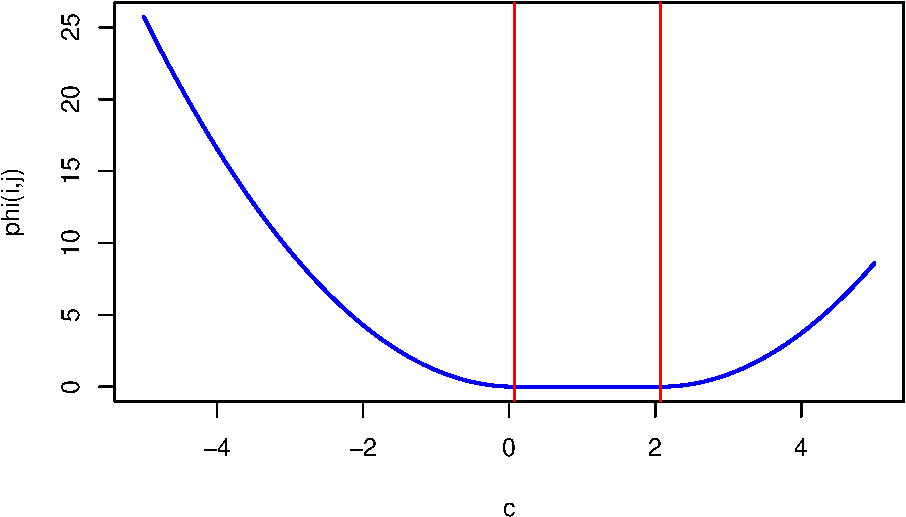
\includegraphics{smacofAC_files/figure-latex/onefunc-1.pdf}
\caption{\label{fig:onefunc}De Gruijter Example, One Phi\_ij}
\end{figure}

Since \(\phi\) is a positive linear combination of the \(\phi_{ij}\) it is also piecewise quadratic, convex, and continuously differentiable
with a continuous piecewise linear increasing derivative. Note \(\phi\) is \textbf{not} twice-differentiable
and \textbf{not} strictly convex. Figure \ref{fig:morefunc} has a plot of \(\phi\) for the De Gruijter
example. The red vertical line is at \(c=c_0\).

\begin{figure}
\centering
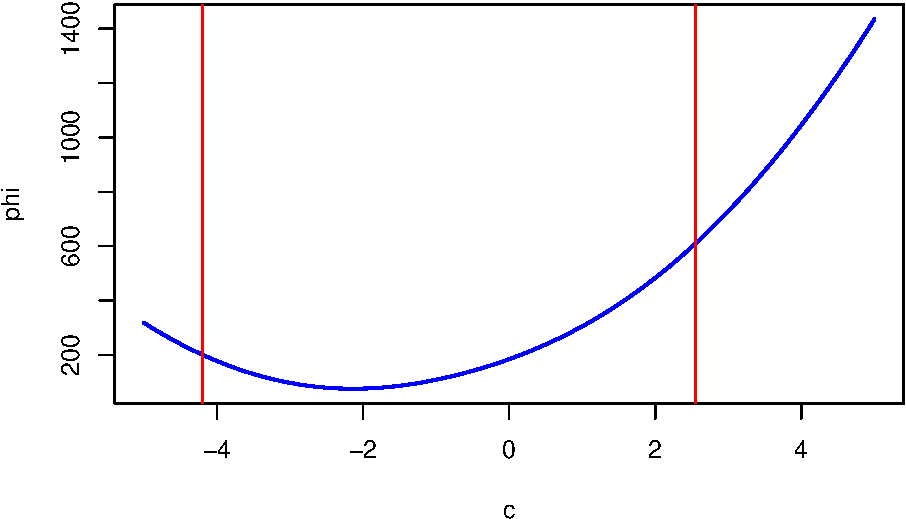
\includegraphics{smacofAC_files/figure-latex/morefunc-1.pdf}
\caption{\label{fig:morefunc}Function Phi for De Gruijter Example}
\end{figure}

We minimize \(\phi\) by using the R function optimize(). From \eqref{eq:derivs} we see that
if \(c\geq\max d_{ij}(X)-\delta_{ij}^-\) then \(\mathcal{D}\phi(c)\geq 0\). This can be used
for the right endpoint of the interval over which we minimize \(\phi\), with \(c_0\) as the left endpoint. The minimum of \(\phi\) in our example turns out to be 75.251647, attained at \(c\) equal to
-2.1403321. The Shepard plot corresponing with the optimum \(c\) is plotted in figure \ref{fig:optbandplot}.

\begin{figure}

{\centering 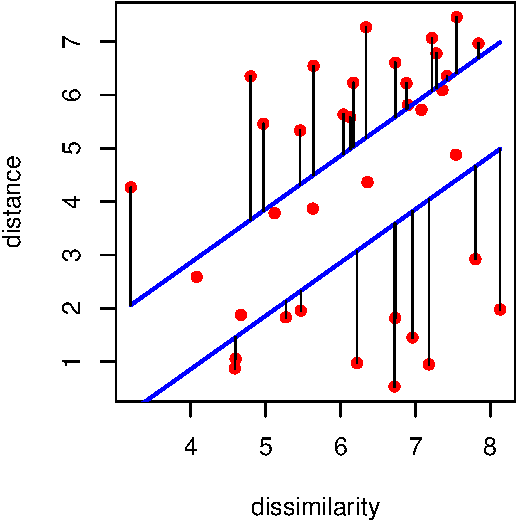
\includegraphics{smacofAC_files/figure-latex/optbandplot-1} 

}

\caption{De Gruijter Shepard Plot}\label{fig:optbandplot}
\end{figure}

\begin{figure}

{\centering 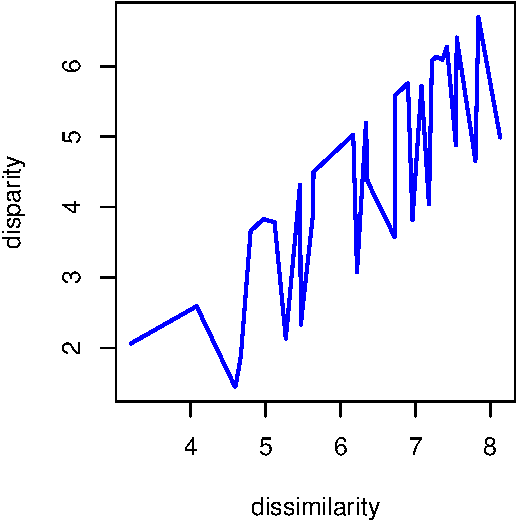
\includegraphics{smacofAC_files/figure-latex/ddhatplot-1} 

}

\end{figure}

\section{Example}\label{example}

\subsection{Type AC4}\label{type-ac4}

\begin{center}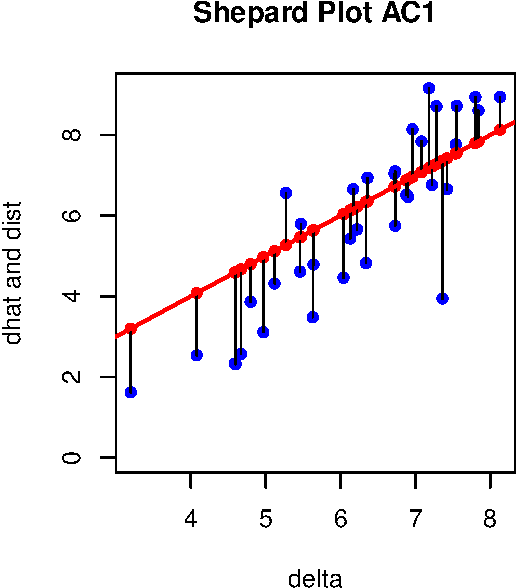
\includegraphics{smacofAC_files/figure-latex/gruijterh00-1} \end{center}

\begin{center}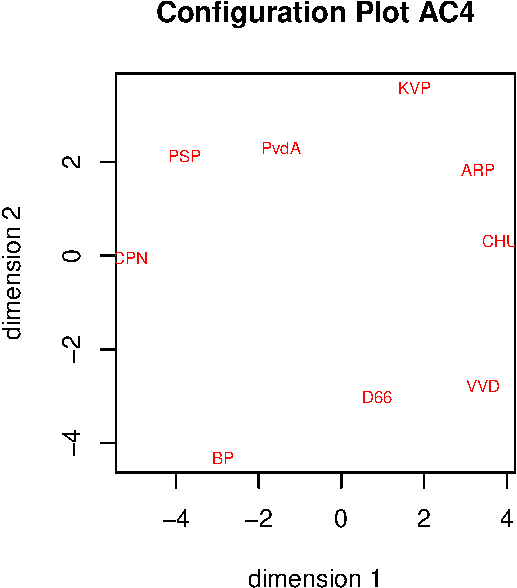
\includegraphics{smacofAC_files/figure-latex/gruijterh00-2} \end{center}

\begin{center}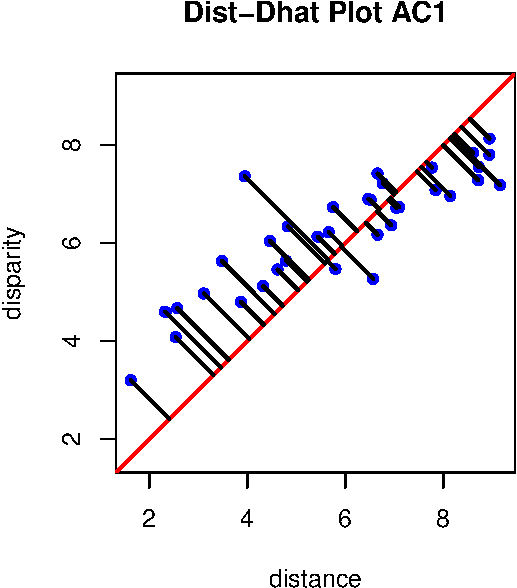
\includegraphics{smacofAC_files/figure-latex/gruijterh00-3} \end{center}

\subsection{Type AC3}\label{type-ac3}

\begin{center}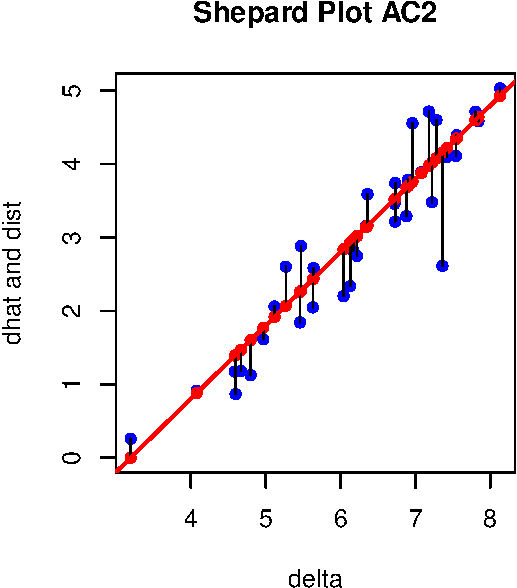
\includegraphics{smacofAC_files/figure-latex/gruijterh10-1} \end{center}

\begin{center}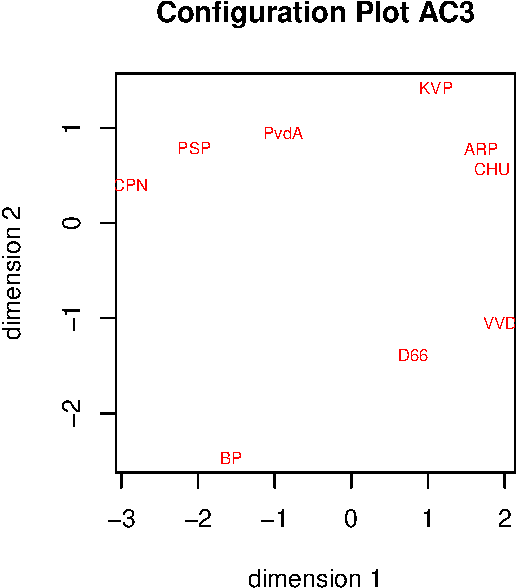
\includegraphics{smacofAC_files/figure-latex/gruijterh10-2} \end{center}

\begin{center}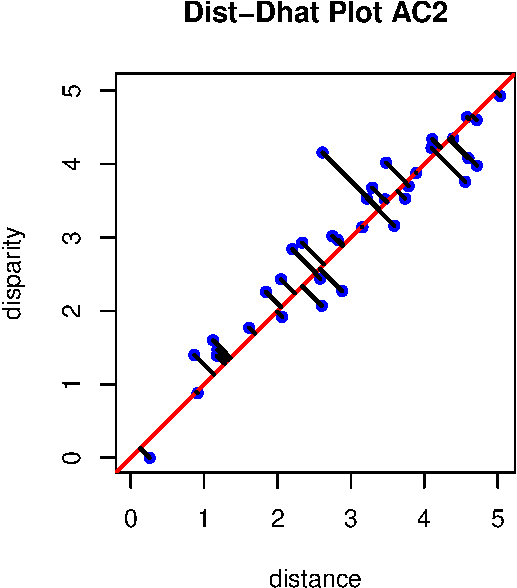
\includegraphics{smacofAC_files/figure-latex/gruijterh10-3} \end{center}

\subsection{Type AC2}\label{type-ac2-1}

\begin{center}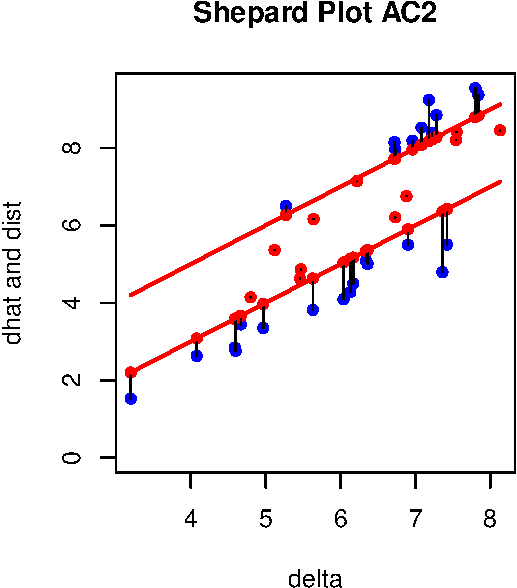
\includegraphics{smacofAC_files/figure-latex/gruijterh01-1} \end{center}

\begin{center}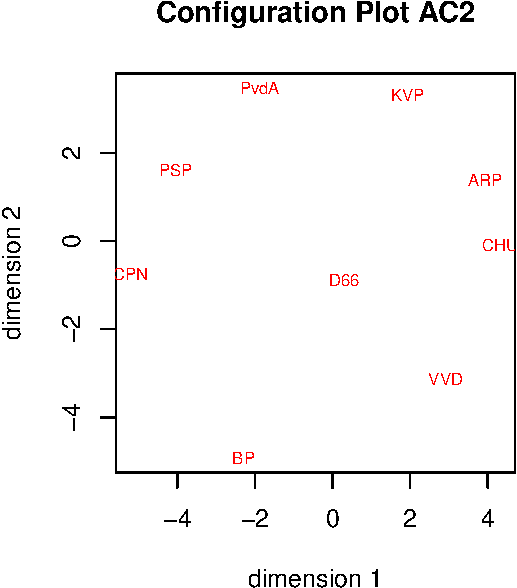
\includegraphics{smacofAC_files/figure-latex/gruijterh01-2} \end{center}

\begin{center}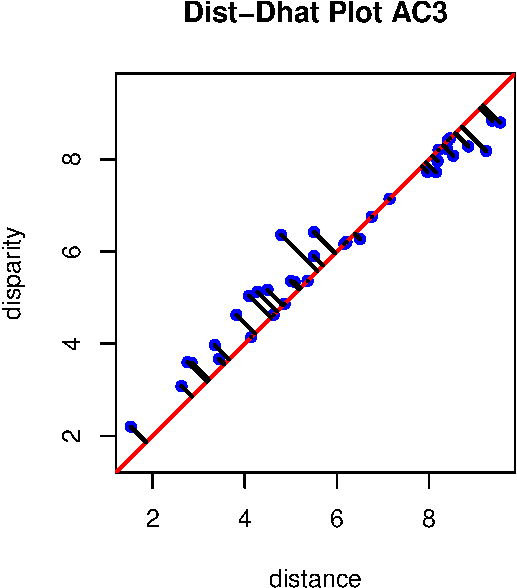
\includegraphics{smacofAC_files/figure-latex/gruijterh01-3} \end{center}

\subsection{Type AC1}\label{type-ac1-1}

\begin{center}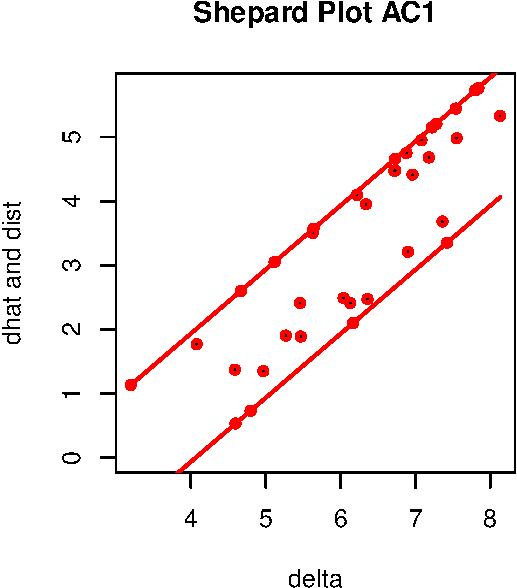
\includegraphics{smacofAC_files/figure-latex/gruijterh11-1} \end{center}

\begin{center}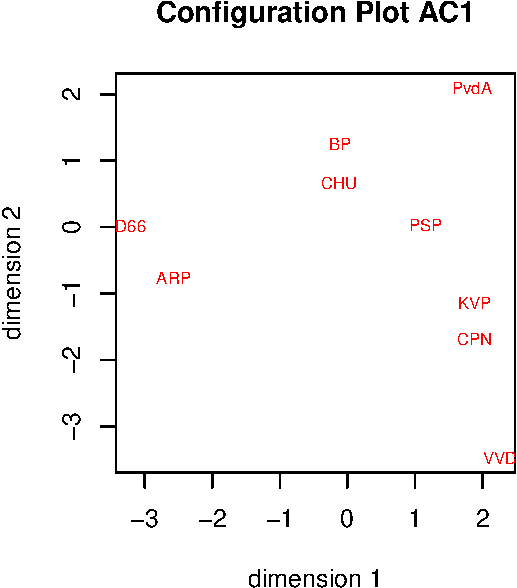
\includegraphics{smacofAC_files/figure-latex/gruijterh11-2} \end{center}

\begin{center}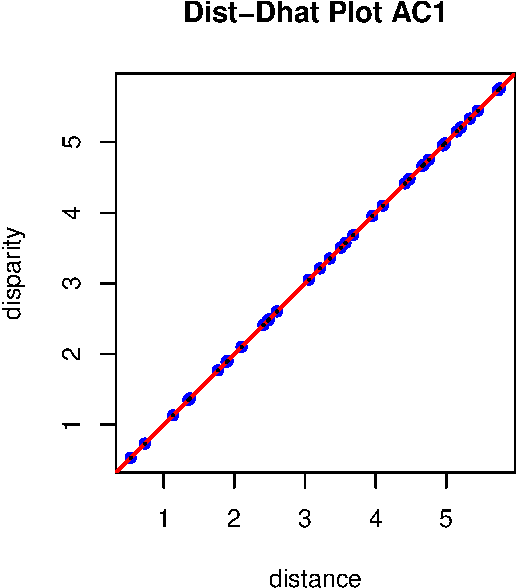
\includegraphics{smacofAC_files/figure-latex/gruijterh11-3} \end{center}

\section*{References}\label{references}
\addcontentsline{toc}{section}{References}

\phantomsection\label{refs}
\begin{CSLReferences}{1}{0}
\bibitem[\citeproctext]{ref-cooper_72}
Cooper, L. G. 1972. {``{A New Solution to the Additive Constant Problem in Metric Multidimensional Scaling}.''} \emph{Psychometrika} 37 (3): 311--22.

\bibitem[\citeproctext]{ref-messick_abelson_56}
Messick, S. J., and R. P. Abelson. 1956. {``{The Additive Constant Problem in Multidimensional Scaling}.''} \emph{Psychometrika} 21 (1--17).

\end{CSLReferences}

\end{document}
